% !TEX TS-program = pdflatex
% !TEX encoding = UTF-8 Unicode

% TeX-M (r1.1)
% For my math classes at UT Austin
% Notes template created by Abdon Morales for the College of Natural Science
% and for the Department of Mathematics and Computer Science
% (c) 2019 - 2024 Abdon Morales and the University of Texas at Austin
% This is a notes template for a LaTeX document using the "article" class for Mathematics (Calculus)
% at the University of Texas at Austin.

% Last change made: Jan 27, 2024 1:40 AM CST

% See "book", "report", "letter" for other types of document.

\documentclass[11pt]{article} % use larger type; default would be 10pt

% Start of Article customization options and addons (for more help and information reference to Overleaf's guides and docs on Latex.
\usepackage[utf8]{inputenc} % set input encoding (not needed with XeLaTeX)

%%% Examples of Article customizations
% These packages are optional, depending whether you want the features they provide.
% See the LaTeX Companion or other references for full information.

%%% PAGE DIMENSIONS
\usepackage{geometry} % to change the page dimensions
\geometry{letterpaper} % or letterpaper (US) or a5paper or....
% \geometry{margin=2in} % for example, change the margins to 2 inches all round
% \geometry{landscape} % set up the page for landscape
%   read geometry.pdf for detailed page layout information

\usepackage{graphicx} % support the \includegraphics command and options
\usepackage{xcolor}

% \usepackage[parfill]{parskip} % Activate to begin paragraphs with an empty line rather than an indent

%%% PACKAGES
\usepackage{booktabs} % for much better looking tables
\usepackage{array} % for better arrays (eg matrices) in maths
\usepackage{paralist} % very flexible & customisable lists (eg. enumerate/itemize, etc.)
\usepackage{verbatim} % adds environment for commenting out blocks of text & for better verbatim
\usepackage{subfig} % make it possible to include more than one captioned figure/table in a single float
\usepackage{exercise}
% Math tools
\usepackage{mathtools}
\usepackage{amsmath}
\usepackage{tikz} % For charts, mathematical graphs, and etc
%% Equal symbol for L'Hospital Rule
\usepackage{tcolorbox}
\newcommand\LR{\stackrel{\mathclap{\normalfont\mbox{L.R}}}{=}}
% These packages are all incorporated in the memoir class to one degree or another...

%%% HEADERS & FOOTERS
\usepackage{fancyhdr} % This should be set AFTER setting up the page geometry
\pagestyle{fancy} % options: empty , plain , fancy
\renewcommand{\headrulewidth}{0pt} % customise the layout...
\lhead{}\chead{}\rhead{}
\lfoot{}\cfoot{\thepage}\rfoot{}

%%% SECTION TITLE APPEARANCE
\usepackage{sectsty}
\allsectionsfont{\sffamily\mdseries\upshape} % (See the fntguide.pdf for font help)
% (This matches ConTeXt defaults)

%%% ToC (table of contents) APPEARANCE
\usepackage[nottoc,notlof,notlot]{tocbibind} % Put the bibliography in the ToC
\usepackage[titles,subfigure]{tocloft} % Alter the style of the Table of Contents
\renewcommand{\cftsecfont}{\rmfamily\mdseries\upshape}
\renewcommand{\cftsecpagefont}{\rmfamily\mdseries\upshape} % No bold!
%%% END Article customizations

%%% The "real" document content comes below...

% Replace examples with the actual content you intend to put
\title{Fiscal Policy \\ Introduction to Macroeconomics}
\author{Abdon Morales \\ The University of Texas at Austin \\ ECO 304L \\ Wayne Geerling}
\date{\today \\ Chapter 16 : Week 10}
%\date{} % Activate to display a given date or no date (if empty),
         % otherwise the current date is printed 

\begin{document}
\maketitle
\subsection*{The Government uses fiscal policy to boost the economy.}
Unlike other recessions, the coronavirus recession began on a date we can pinpoint: March 11, 2020. That was the day many sectors in the U.S economy shut down and people began social distancing in earnest. The federal government instituted border closures and other travel restrictions; restaurants started to doing take-out business only, theme parks closed, colleges sent their students home, in sport, the NBA and PGA suspended play mid-season and the NCAA's "March Madness" basketball tournament was canceled. Most type of business were allowed to stay open, but since masks, hand sanitizer, and COVID-19 test kits were scarce, many closed anyway out of concern for the safety of their staff and customers. The stock market responded to all this turmoil with a massive one-day drop quickly dubbed "Black Thursday".

It was immediately clear that the many people and businesses suffering from the shutdowns would need help. Over the next two months, Congress passed, and the president signed, spending packages adding up to more than \$2.5 trillion. Included were tax rebates and unemployment compensation for individuals, and various kinds of assistance for businesses and state and local governments; billions of dollars were earmarked for hard-hit industries like airlines and hospitals.

In this chapter, we consider how economists expect fiscal policy to affect the economy. We begin by discussing traditional demand-side fiscal policy in the aggregate demand-aggregate supply model. We then consider the potential shortcomings of this approach to fiscal policy; finally, we consider fiscal policy focused on aggregate supply, which can be more effective when economic problems lie primarily on the supply side of the economy. This happened during the coronavirus pandemic.

\begin{tcolorbox}[width=\textwidth,colback={white},title={Big Questions},colbacktitle=yellow,coltitle=blue]
\begin{itemize}
\item What is fiscal policy?
\begin{itemize}
\item Fiscal policy involves the use of government's budget tools, government spending, and taxes to influence the macroeconomy, often through aggregate demand.
\item Countercyclical fiscal policy is designed to counteract business cycle fluctuations by increasing aggregate demand during downturns and decreasing aggregate demand during expansionary periods.
\end{itemize}
\item What are the shortcomings of fiscal policy?
\begin{itemize}
\item Fiscal policy is subject to three significant lags: a recognition lag, an implementation lag, and an impact lag.
\item In addition, crowding-out can diminish the effects of fiscal policy.
\item Finally, according to the new classical critique, savings adjustments by private individuals can further diminish the stimulating effects of fiscal policy.
\end{itemize}
\item What is supply-side fiscal policy?
\begin{itemize}
\item Supply-side fiscal policy involves the use of government spending and taxes to affect the production (supply) side of the economy. This is a long-run view that concentrates on institutional changes.
\item A key proposal of supply-side fiscal policy is that lower marginal income tax rates can actually lead to greater tax revenue when tax rates are high.
\end{itemize}
\end{itemize}
\end{tcolorbox}

\section*{\textbf{What is fiscal policy?}}
When the economy falters, people often look to government to help push the economy forward again. In fact, the government uses many different tools to try to affect the economy. Economists sort these into two types of policy: \textit{monetary policy} and \textit{fiscal policy}; monetary policy is the use of the money supply to influence the economy (we will study monetary policy in Chapter 18). \textbf{\textcolor{red}{Fiscal policy}}, the subject of this chapter, involves the use of government budget tools, spending, and taxes to influence the macroeconomy. In the United States, tax and spending changes are legislated and approved by both Congress and the president.

In this section, we first describe how the government can use fiscal policy to try to simulate the economy; then we discuss how fiscal policy might be used to slow down rapid growth. Along the way, we consider how fiscal policy affects government budget deficits and debt; finally, we examine the multiplier process, which describes the ways in which the effects of fiscal policy riple through the economy.

\subsection*{\textbf{\textit{Expansionary Fiscal Policy}}}
Fiscal policy is typically focused on the spending or demand side of the economy. Private spending generally falls during recessions, so people look to the government to spend some more and also to cut taxs to encourage private spending. \textbf{\textcolor{red}{Expansionary fiscal policy}} occurs when the government increases spending or decreases taxes to stimulate the economy toward expansion. In this section, we use the aggregate demand-aggregate supply model to examine the effects of expansionary fiscal policy.

In Chapter 13, we introduced the aggregate demand-aggregate supply model; in that model, we showed that recession can occur as a result of a drop in aggregate demand. In theory, the econony can move itself back to full employment in the long run when all prices adjust.

In addition, recessions are difficult times for many people, and they expect the government to take action to ease their pligth. Thus, government officials often choose to use fiscal policy to try and shift aggregate demand back to its original level. If they're policy works, the economy returns to full-employment equilibrium.
\begin{center}
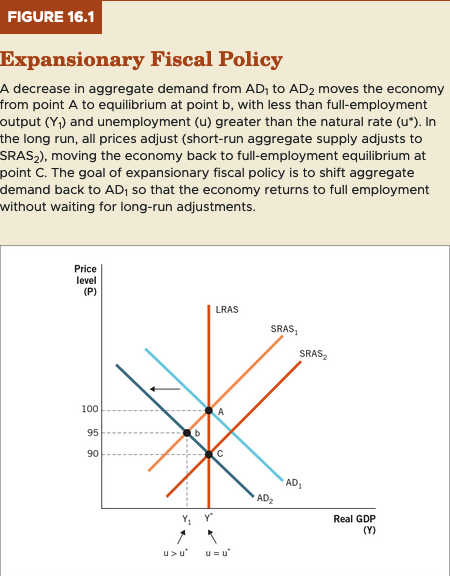
\includegraphics[scale=0.5]{images/Figure 16.1.png} 
\end{center}
Fiscal policy can make use of government spending, taxes, or a combination of the two. Recall that aggregate demand has four pieces: consumption (C), investment (I), government spending (G), and net exports (NX). Therefore, increases in G directly increase aggregate demand; when private spending (consumption, investment, and net exports) is low, the government can increase demand directly by increasing G. Fiscal policy can also focus on consumption (C) by decreasing taxes; decreases in taxes can increase aggregate demand because people have more of their income left to spend after paying their taxes. When peopl keep more of their pay check, they can afford more consumption.

\begin{center}
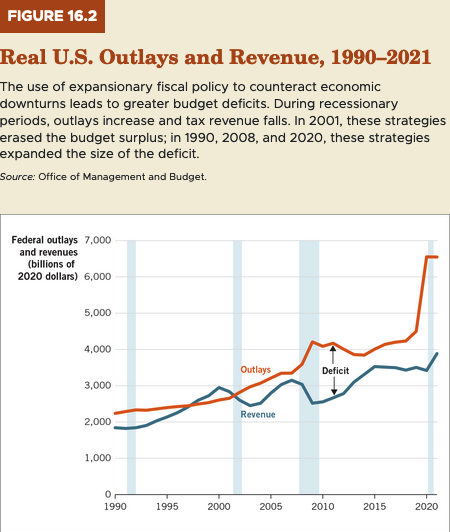
\includegraphics[scale=0.5]{images/Figure 16.2.png} 
\end{center}

The bottom line is clear: expansionary fiscal policy inevitably leads to increases in budget deficits and the national debt during economic downturns. This policy prescription may seem odd; after all, if you personally fell on rough economic times, you might (reasonably) react differently. For example, if your employer were to cut you back from full-time to part-time employment, would it seem like a good idea to go on a spending binge? You might feel better while you were shopping, but it woudln't help your financial situation much. From a macroeconomic perspective, however, expansionary fiscal policy might work for the overall economy because spending by one person becomes income to another, which can snowball into income increases throughout the economy. We discuss this "multiplier" aspect of fiscal policy later in this chapter.

\subsection*{\textbf{\textit{Contractionary Fiscal Policy}}}
We have seen that expansionary fiscal policy is often used to try to increase aggregate demand during economic downturns; but there are also times when contractionary fiscal policy is used to reduce aggregate demand. \textbf{\textcolor{red}{Contractionary fiscal policy}} occurs when the government decreases spending or increases taxes to slow economic expansion.

There are two reasons why a government might want to reduce aggregate demand. First, as we discussed earlier, expansionary fiscal policy creates deficits during recessions; an increase in taxes or a decrease in spending during an economic expansion can work to reduce the budget deficit and pay off some government debt.
Second, the government might want to reduce aggregate demand if it believes that the economy is expanding beyond its long-run capabilities. Full-employment output ($Y$*) is considered the highest level of output sustainable in the long run; but if the unemployment rate falls below the natural rate ($u$*), output may be above $Y$*. Some economists then worry that the economy may "overheat" from too much spending, which can lead to inflation.

\begin{center}
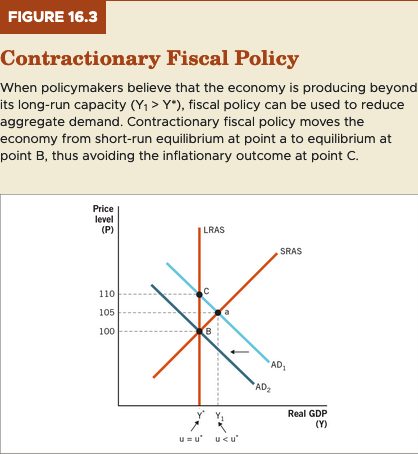
\includegraphics[scale=0.5]{images/Figure 16.3.png} 
\end{center}

Together, contractionary and expansionary fiscal policy can serve to counteract the ups and downs of business cycles. We examine this combination more closely in the next section.

\subsubsection*{\textit{Countercyclical fiscal policy}}
\subparagraph*{All else being equal, people generally prefer smoothness and predictability in their financial affairs. In Chapter 9, we talked about this characteristic in reference to consumption smoothing; in Chapter 10, we considered how people are risk averse. Along these lines, an economy that grows at a consistent rate is preferable to an economy that grows in an erratic fashion. \\Fiscal policy that seeks to counteract business cycle fluctuations is known as \textbf{\textcolor{red}{countercyclical fiscal policy}}. It consists of using expansionary policy during economic downturns and contractionary policy during economic expansions. Figure 16.4 illustrates the goals of countercyclical fiscal policy; the natural path of the economy (without countercyclical fiscal policy) includes business cycles during which income and employment fluctuate. The goal of countercyclical fiscal policy is to reduce those fluctuations. \\You might recall from Chapter 14 that Keynesian economists focus on aggregate demand (total spending) in the economy. Keynesian economics provides the theoretical foundation for countercyclical fiscal policy.\\Table 16.1 summarizes the tools of countercyclical fiscal policy, including the timing and effects of the policy on aggregate demand as well as its effects on the government budget deficit. In practice, while politicians are quick to reach for expansionary tools during economic downturns, they are much less quick to reach for contractionary tools in boom times. \textbf{\textit{Expansionary policy is popular; contractionary policy isn't.}}}
\begin{center}
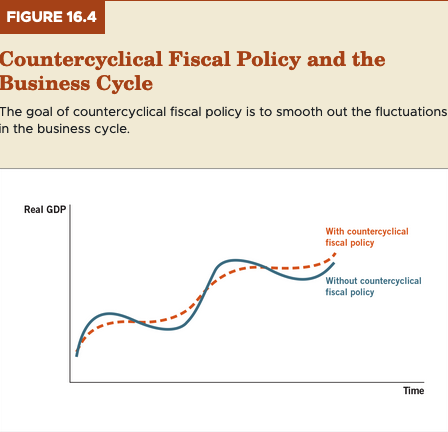
\includegraphics[scale=0.5]{images/Figure 16.4.png} 
\end{center}

\subsection*{Multipliers}
The tools of fiscal policy are possibly more powerful than our discussion thus far implies, because the initial effect can snowball overtime. When fiscal policy shifts aggregate demand, some effects are felt immediately; but a large share of the impact occurs later as spending effects ripples throughout the economy. To see this process clearly, we need to build on two concepts we learned in previous chapters. One should be familiar; the other is new.

\begin{center}
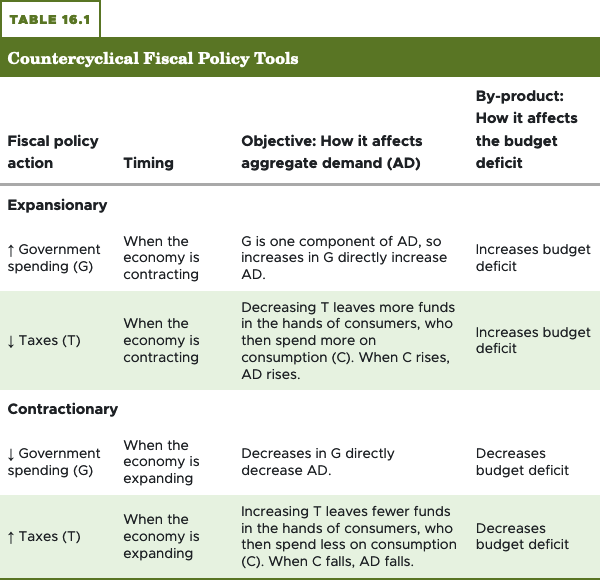
\includegraphics[scale=0.5]{images/Table 16.1.png} 
\end{center}

First, the familiar concept: recall from Chapter 6 that spending by one person becomes income to others. This is true not only for private spending but also for government spending.

Now the new concept: increases in income generally lead to increases in consumption. When a person's income rises, he or she might save some of this new income but might be just as likely to spend part of it, too. The \textbf{\textcolor{red}{marginal prosperity to consume (MPC)}} is the portion of additional income spent on consumption:
\begin{equation}
\text{MPC} = \frac{\text{change in consumption}}{\text{change in income}}
\end{equation}
\textit{\textcolor{red}{The multiplier effect is significant when we focus on aggregate demand in the economy. Each time people earn new income, they spend part of it.} After all the dust settles, the total effect is a multiple of the original fiscal policy spending.}

In the graph, we show aggregate demand; each time spending increases, aggregate demand increases (shifts rightward). The initial aggregate demand is labeled $\text{AD}_1$; each round of spending shifts aggregate demand to the right by less and less, until aggregate demand settles at $\text{AD}_N$, where $N$ represents the completetion of the multiplier process.

\begin{center}
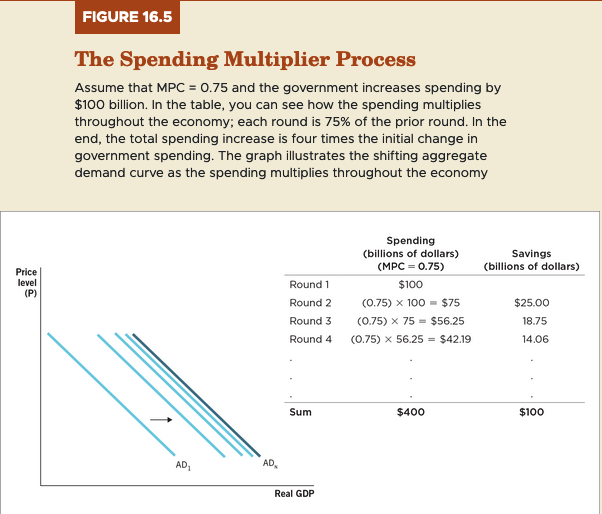
\includegraphics[scale=0.5]{images/Figure 16.5.png} 
\end{center}

To determine the total effect on spending from any initial government expenditures, we use the \textit{\textcolor{blue}{spending multiplier}}. The \textbf{\textcolor{red}{spending multiplier}} ($m^s$) tells us the total impact on spending from an initial change of a given amount. The multiplier depends on the marginal propensity to consume: the greater the marginal propensity to consume, the greater the spending multiplier. The formula for the spending multiplier is
\begin{equation}
m^s=\frac{1}{1-\text{MPC}}
\end{equation}
Because the MPC is a fraction between 0 and 1, in principle the multiplier must come out larger than 1. Sometimes, the spending multiplier is called the \textit{\textcolor{blue}{Keynesian multiplier}} or \textit{\textcolor{green}{fiscal multiplier}}.

Note that the multiplier concept applies to all spending, no matter whether the spending is public or private. In addition, there is a multiplier associated with tax changes; a reduction in tax rate leaves more income for consumers to spend. This spending multiplies throughout the economy in much the same way as government spending multiplies.

The multiplier process also works in reverse; if the government reduces spending or increases taxes, people have less income to spend, shifting the aggregate demand curve to the left. In terms of the aggregate demand curve in Figure 16.5, the initial decline in government spending leads to subsequent declines as the effects reverberate through the economy.

In theory, then, the spending multiplier implies that the tools of fiscal policy are very powerful. Not only can the government change its spending and taxing, but multiples of this spending then ripple throughout the economy over several periods. In reality, however, government spending multipliers are not very large; the largest multipliers occur with temporary deficit-financed increases in government spending, but even these rarely go above 1.5. Even more surprisingly, Valerie Ramey, an economist at the University of California, San Diego (UCSD), estimates that multipliers are typically less than 1 - not something you'd expect based on how we derived the multiplier form the MPC. This implies that government spending increases don't always translate into more overall spending. In the next section, we cover this more fully, as we discuss shortcomings of fiscal policy.

\section*{\textbf{What are the shortcomings of fiscal policy?}}
At this point, you may wonder why fiscal policy doesn't always work perfectly in the real world. If fiscal policy is as simple as tweaking government spending and taxes and letting the multiplier go to work, why do recessions still happen? The first answer is that the real world isn't so simple; millions of people make individual decisions that collectively affect the entire economy. While economists try to forecast variables and outcomes (how much will people spend versus save?), they can never be certain of the answers to these questions ahead of time. Even the most informed and educated guesses are sill guesses and not guarantees.

But there are also more specific shortcomings of fiscal policy; in this section, we consider three issues that arise in the application of fiscal policy: time lags, crowding out, and savings shifts.

\subsection*{\textit{\textbf{Time Lags}}}
Economic policy is intended to smooth out the economic variations that accompany a business cycle, so timing is important. But there are three time lags that accompany policy decisions: recognition lag, implementation lag, and impact lag.
\begin{itemize}
\item \textit{\textcolor{blue}{Recognition lag}}. In the real world, it is difficult to determine when the economy is turning up or down. GDP data are released quarterly, and the final estimate for each quarter is not know until three months after the period in question. In addition, it often takes a while for unemployment rates to reflect macroeconomic conditions, moreover, growth is not constant: one bad quarter does not always signal a recession, and one good quarter is not always the beginning of an expansion. All these factors make it hard to recognize turns in the business cycle.
\item \textit{\textcolor{blue}{Implementation lag}}. It also takes time to implement fiscal policy; in most nations, one or more governing bodies must approve tax and spending legislation. In the United States, such legislation must pass both houses of Congress and receive presidential approval before becoming law. For this reason, fiscal policy takes much longer to implement than monetary policy.
\item \textit{\textcolor{blue}{Impact Lag}}. Finally, it takes time for the complete effects of fiscal or monetary policy to materialize. The multiplier makes fiscal policy powerful, but it takes time to ripple through the economy.
\end{itemize}

If lags causes the effects of fiscal policy to be delayed for a year or 18 months, there is a risk that the policy can actually magnify the business cycle. That is, if the effects of expansionary fiscal policy hit when the economy is already expanding, the result may be excessive aggregate demand and inflation; and if contractionary fiscal policy is implemented and followed by time lags, the effects could be lead to even deeper recessions.

\subsubsection*{\textit{Automatic Stabilizers}}
\subparagraph*{One possibility of alleviating lag problems are programs that automatically adjust government spending and taxes when economic conditions change. \textbf{\textcolor{red}{Automatic stabilizers}} are government programs that automatically implement countercyclical fiscal policy in response to economic conditions. Given that the prescription is to increase spending and increase taxes during expansions, there are several government programs that accomplish these goals automatically:}
\begin{itemize}
\item \textit{\textcolor{teal}{Progressive income tax rates}} guarantee that individual tax bills fall when incomes fall (during recessions) and rise when incomes rise (during expansions).
\item \textit{\textcolor{teal}{Taxes on corporate profits}} lower total tax bills when profits are lower (during contractions) and raise tax bills when profits are higher (typically during expansions).
\item \textit{\textcolor{teal}{Unemployment compensation}} increases government spending automatically when the number of unemployed people rises and decreases government spending when fewer people are unemployed.
\item \textit{\textcolor{teal}{Welfare programs}} also increase government spending during downturns and decreases government spending when the economy is doing better.
\end{itemize}
\subparagraph*{In short, automatic stabilizers can eliminate recognition lags and implementation lags about thereby alleviate some concerns about the destabilizing effects of fiscal policy.}

\subsection*{\textit{\textbf{Crowding-Out}}}
A second challenge in implementing fiscal policy concerns the actual impact of government spending and the multiplier effects. Unfortunately, increases in government spending can lead to decreases in private spending; when government spending substitutes for private spending, the overall change in aggregate demand diminishes. Economists call this effect \textbf{\textcolor{red}{crowding-out}}. It occurs when private spending falls in response to increases in government spending.

When crowding-out occurs, aggregate demand does not increase as anticipated, and the fiscal policy is less effective.

Let's look more closely at how crowding-out can work; first, for simplicity, assume that the nation has a balanced government budget and a closed economy (no import or exports). Now suppose the government increases spending by \$100 billion but does not raise taxes. This means it must borrow the \$100 billion in the loanable funds market, but as we know, every dollar borrowed requires a dollar saved. So when the government borrows \$100 billion, the money has to come from \$100 billion in savings.

\begin{center}
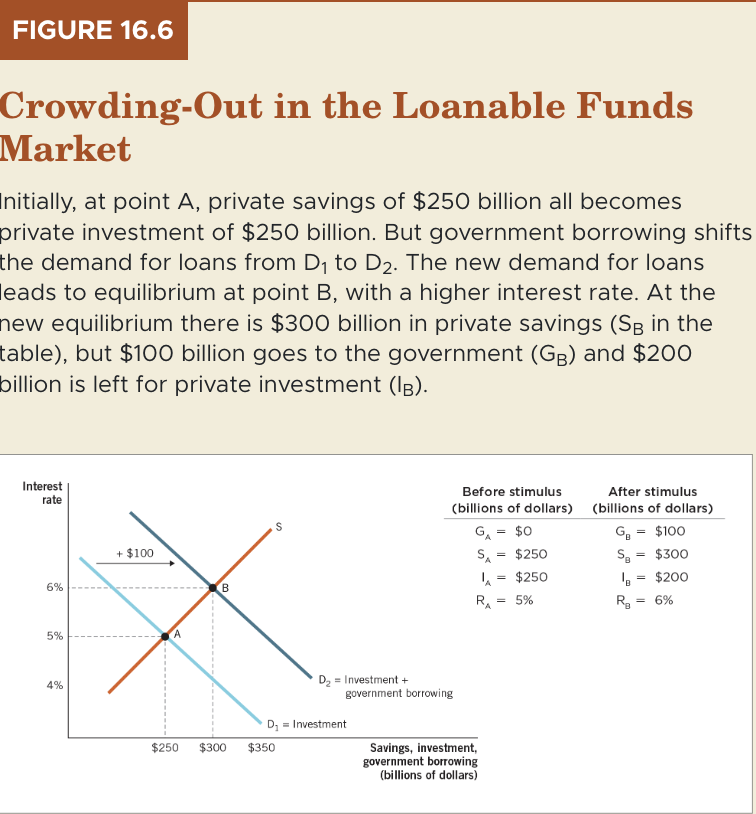
\includegraphics[scale=1]{images/Figure 16.6.png} 
\end{center}

\subsection*{\textit{\textbf{Savings shift}}}
New spending today has to be paid for someday, which means that taxes must rise sooner or later. The \textbf{\textcolor{red}{new classical critique}} of fiscal policy, a model developed in the 1970s by a group of economists including Nobel Prize winners Robert Barro, Robert Lucas, and Thomas Sargent, asserts that increases in government spending and decreases in taxes are largely offset by increases in savings, because people know they'll have to pay higher taxes eventually. But if savings increases, consumption falls, and this outcome mitigates the positive effects of the government spending.

Table 16.2 summarizes the three shortcomings that can diminish the effects of fiscal policy.

\begin{center}
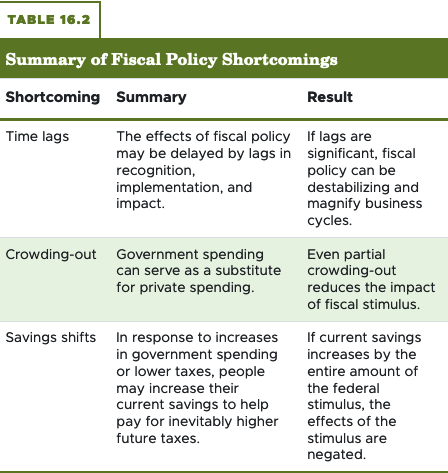
\includegraphics[scale=0.5]{images/Table 16.2.png} 
\end{center}

\section*{What is supply-side fiscal policy?}
We have considered typical fiscal policy, which focuses squarely on aggregate demand. It is also possible to implement fiscal policy with the intent of affecting the supply side of the economy. In this section, we begin by describing the supply-side perspective and certain popular supply-side policy proposals. We then look more closely at marginal tax rates and consider how changes in tax rates can affect the economy.

\subsection*{\textbf{\textit{Supply-focused fiscal policy in the coronavirus recession}}}
In April of 2020, as the COVID-19 spread through the United States, the unemployment rate spiked to 14.7\%. However, it came down over the next few months and was back in single-digit territory by August. Most economists attribute the rapid turnaround to government actions that targeted both aggregate demand and aggregate supply.

As we discussed in Chapter 14, the initial economic effects of the virus were primarily on the supply side of the economy: it became more expensive to produce just about anything, as businesses had to incorporate protocols involving masks, social distancing, frequent cleaning and disinfection, and regular COVID-19 testing into their production methods. In that situation, it made sense for the government to try and shore up the supply side of the economy. The use of government spending and taxes for this purpose is called \textbf{\textcolor{red}{supply-side fiscal policy}}.

The supply side is where decisions are made on what to produce, and how much, given available resources, institutions, and technology. Economic changes that increase production costs for a broad range of suppliers will reduce aggregate supply.

In the Spring of 2020, three separate fiscal policy acts were passed on Capital Hill and signed by President Trump. The total price tag for these was over \$2.5 trillion, more than double the cost of any previous U.S fiscal policy, even after adjustment for inflation; but these spending bills were different from the government's actions during the Great Recession, described earlier. This time, much of the aid was supply-side spending, which went directly to businesses. The major provisions of these acts included:
\begin{enumerate}
\item \textit{\textcolor{olive}{Small business grants}}. The Paycheck Protection Program (PPP) was a \$659 billion initiative that extended loans to small businesses to help them survive the shutdown periods. Importantly, these loans were forgiveable (they could convert to cash grants) if firms used the funds to retain workers during the downturns. The goal was to minimize layoffs by helping pay workers' wages.
\item \textit{\textcolor{olive}{Loans to airlines and other large corporations}}. Because firms and households depend heavily on air travel, keeping airlines from failing made sense in a way of speeding economic recovery. Loans to other big corporations were, like the loans to small businesses, intended to minimize the number of workers laid off.
\item \textit{\textcolor{olive}{Hospital aid}}. During the pandemic, many hospitals reduce their admittance of nonemergency patients to make room for COVID-19 emergencies. This created a cash-flow problem for hospitals, rigth when their services were needed most; federal aid went directly to hospitals to keep them afloat.
\item \textit{\textcolor{olive}{State and local government aid}}. States, counties, and cities had many additional expenses associated with virus testing and tracing, so they also received needed aid.
\item \textit{\textcolor{olive}{Tax rebates}}. Households that earned less than \$75,000 in 2019 received a tax rebate of \$1,200 per single person or \$2,400 per couple, and additional \$500 per child.
\item \textit{\textcolor{olive}{Unemployment compensation}}. In addition to unemployment compensation from existing state programs, laid-off workers received federal benefits in the amount of \$600 per week.
\end{enumerate}

Of the six components, the first four focused on the supply side of the economy, while the last two focused on aggregate demand.

\begin{center}
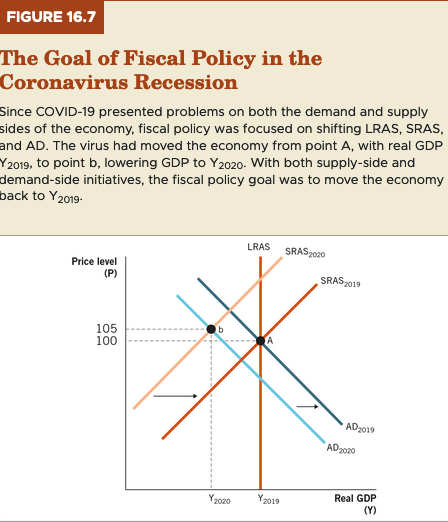
\includegraphics[scale=0.5]{images/Figure 16.7.png}
\end{center}

\subsection*{\textbf{\textit{Other Supply-Focused Fiscal Policy}}}
Many other fiscal policy initatives are designed to focus on the supply side of the economy. These include:
\begin{enumerate}
\item \textit{\textcolor{lime}{Research and development (R\&D) tax credits}}. Tax breaks are given to firms that spend resources to develop new technology; for example, if an atlernative energy firm spends resources on a new lab to develop alternative energy sources, this spending reduces its overall tax bill.
\item \textit{\textcolor{lime}{Policies that focus on education}}. Subsidies or tax breaks for education expenses are given to help create incentives to invest in education. One example is the Pell Grant, which helps to pay for college expenses; student receive these grants from the federal government to help them pay for college education. Eventually, education and training increase effective labor resources and thus increase aggregate supply.
\item \textit{\textcolor{lime}{Lower corporate profit tax rates}}. Lower taxes increases the incentives for corporations to undertake activities that generate more profit.
\item \textit{\textcolor{lime}{Lower marginal income tax rates}}. Lower income tax rates create incetives for individuals to work harder and produce more, because they keep a larger share of their income. We discuss marginal tax rates in the next section.
\end{enumerate}

All of these initiatives share two characteristics: first, they increase incentives for productive activities. Second, each initiative takes time to affect aggregate supply. For example, education subsidies may encourage people to go to college and learn skills useful in the workplace; but the full effect of that education isn't felt until after the education is completed. For this reason, supply-side proposals are generally emphasized as long-run solutions to growth problems.

\subsection*{\textbf{\textit{Marginal income tax rates}}}
We have noted that lowering marginal income tax rates is one way that fiscal policy can affect the supply side of the economy. The relationship between tax rates and tax revenue is, regrettably, highly politicized; on one side of the debate are lobbying firms and other factions that constantly call for lower tax rates, while their counterparts on the other side invariably push for higher tax rates. Careful, ojective economic analysis leads to a more nuanced position; economists recognize that tax revenue is necessary to fund the government activity that citizens need and expect. Economists also recognize that high tax rates disincentivize production and thereby inhibit economic progress. This narrative does not fit nicely into either extreme political camp; this is the section where we look more closely at how tax rates affect incentives for production.

\subsubsection*{\textit{\textcolor{olive}{Tax Rates and Tax Revenue}}}
When tax rates are relatively low, an increase in leads to an increase in tax revenue. At low tax rates, increases in tax rates lead to revenue increases.

But it turns out that if you raise rates too high, tax revenue declines because the high rates provide negative incentives for production. This means that when tax rates are particularly high, a reduction in tax rates could actually lead to an increase in tax revenue. Tax rate cuts can be creative; that is, they can stimulate work effort, employment, and income and thereby generate \textit{more} income tax revenue for the government.

\subsubsection*{\textit{\textcolor{olive}{The Laffer Curve}}}
\subparagraph*{In 1974, University of Chicago professor and economist Arthur Laffer famously tried to illustrate the relationship between tax rates and tax revenue by sketching a drawing on the back of a napkin at dinner. This relationship became known as the Laffer Curve; soon after, it became a centerpiece for Ronald Reagan's presidency (1981 - 1989) in the 1980s and a central component of supply-side economics. Almost since its inception, this curve has been debated.}
\subparagraph*{To understand this curve, let's first clarify the relationship between tax rates and tax revenue. Total income tax revenue depends on the level of income and the tax rate:}
\begin{equation}
\text{income tax revenue}=\text{tax rate}\times \text{income}
\end{equation}
\subparagraph*{This equation is straightforward, but because humans beings react to incentives; it is not always easy to predict how tax revenue will change when tax rates change. The \textbf{\textcolor{red}{Laffer curve}}, shown in Figure 16.8, illustrates the relationship between tax rates and tax revenue. Notice we have labeled two regions of the Laffer curve: Region I, the blue portion leads to increasing tax revenues: 
\begin{equation}
\uparrow \text{income tax revenue} = \uparrow \text{tax rate} \times \text{income}
\end{equation}
}
\subparagraph*{But at some point, tax rates become so high that they provide significant disincentives for earning income. This is the case in Region II, illustrated by the orange portion of the curve, where increases in the tax rate leads to less tax revenue. [$\text{MTR}= <90\%$] At this point, an increase in the tax rate reduces income enough (illustrated by the double downward-pointing arrows) that net tax rate revenue falls:
\begin{equation}
\downarrow \text{income tax revenue} = \uparrow \text{tax rate} \times \downarrow\downarrow \text{income}
\end{equation}
}
\subparagraph*{In region II of the Laffer curve, decreases in the tax rate lead to increases in tax revenue. At the lower rate, people have greater incentives to work and earn income. Thus, the lower tax rates stimulate the economy and lead to more tax revenue overall.
\begin{center}
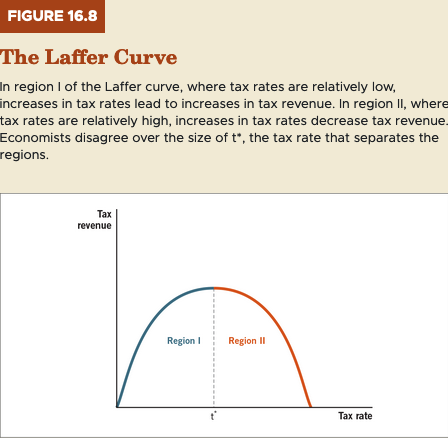
\includegraphics[scale=0.4]{images/Figure 16.8.png} 
\end{center}
}
\subparagraph*{
\begin{center}
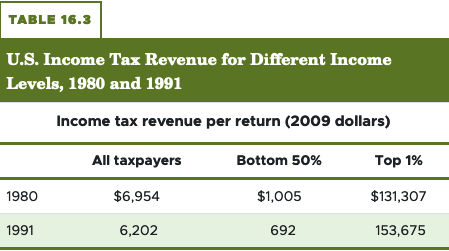
\includegraphics[scale=0.5]{images/Table 16.3.png} 
\end{center}
At some specific tax rate, tax revenue is maximized; in Figure 16.8, this rate is labeled $t$*. Economists don't know exactly what this amount is, but it seems to be less than 70\% in the United States, based on experience from the 1980s. In 1980, the marginal tax rate on the wealthiest Americans was 70\%, but then marginal rates fell across all income brackets over the course of the decade. The result was higher tax revenue from the wealthiest Americans (see Table 16.3) even though tax revenue per taxpayer fell overall. Considering all U.S taxpayers, average tax revenue (adjusted for both inflation and the number of tax returns filed) went from \$6,954 to \$6,202 between 1980 and 1991. Many analysts point to these figures and see them as proof that Laffer curve doesn't exist or even that supply-side economics lacks merit. However, at very high rates, the experience of the 1980s shows that rate reductions can lead to higher revenue.
}
\subparagraph*{Table 16.3 shows data from the 1980s regarding tax revenue from taxpayers at different income levels. The rate reductions led to less tax revenue overall because of drops in tax revenue from the many taxpayers who were paying relatively low taxes to begin with. Overall, revenues declined when we adjust fro both inflation and population, but for the wealthiest Americans, a rate reduction led to an increase in revenue. The takeaway from Table 16.3 is that data from the 1980s confirm the two distinct regions on the Laffer curve. Generally, conservative public figures tend to stress region II, where tax rate reductions lead to increases in revenue; liberals emphasize region I, where tax rate increases lead to more revenue. Recognizing both regions is important for economic policy.}

\section*{Conclusion}
We began this chapter with a recent example of real-life fiscal policy in the United States. Over the next few years, we will be able to see how the 2017 tax cuts actually affected the economy. For sure, the deficit increased, but growth effects will take some time to work out.

Looking ahead, we turn our attention next to monetary policy; in Chapter 17, we cover money and the Federal Reserve, in Chapter 18, we discuss how monetary policy affects the economy.

\end{document}